%
% File tto2019.tex
%
%% Based on the style files for ACL 2019, ACL 2018, NAACL 2018/19, which were
%% Based on the style files for ACL-2015, with some improvements
%%  taken from the NAACL-2016 style
%% Based on the style files for ACL-2014, which were, in turn,
%% based on ACL-2013, ACL-2012, ACL-2011, ACL-2010, ACL-IJCNLP-2009,
%% EACL-2009, IJCNLP-2008...
%% Based on the style files for EACL 2006 by 
%%e.agirre@ehu.es or Sergi.Balari@uab.es
%% and that of ACL 08 by Joakim Nivre and Noah Smith

\documentclass[11pt,a4paper]{article}
\usepackage[hyperref]{tto2019}
\usepackage{times}
\usepackage{latexsym}
\usepackage{graphicx}

\usepackage[labelfont=bf]{caption}

\usepackage{url}

%\aclfinalcopy % Uncomment this line for the final submission

%\setlength\titlebox{5cm}
% You can expand the titlebox if you need extra space
% to show all the authors. Please do not make the titlebox
% smaller than 5cm (the original size); we will check this
% in the camera-ready version and ask you to change it back.

\newcommand\BibTeX{B\textsc{ib}\TeX}

\title{Investigating Facebook's policy against accounts that repeatedly share misinformation: implementation and impact}

\author{Héloïse Théro \\
  médialab - Sciences Po, Paris, France \\
  \texttt{thero.heloise@gmail.com} \\\And
  Emmanuel Vincent \\
  médialab - Sciences Po, Paris, France \\
  \texttt{emmanuel.vincent@sciencespo.fr} \\}

\date{}

\begin{document}
\maketitle

\begin{abstract}
Like many web platforms, Facebook is under pressure to regulate misinformation. 
According to the company, users that repeatedly share misinformation (`repeat offenders') will have their distribution reduced, but little is known about the implementation or the efficiency of this measure.
First, combining data from a fact-checking organization and CrowdTangle, we identified a set of public accounts (groups and pages) that have shared misinformation repeatedly. 
While we observe a decrease in engagement for pages (median of $-43\%$) after they shared two or more `false news', such a reduction is not observed for groups. 
However, we discover that groups have been affected in a different way with a sudden drop in their average engagement per post that occurred around June 9, 2020.
No public information was given by Facebook about this sudden decrease.
This drop has cut the groups’ engagement per post in half, but it was compensated by the fact that the overall activity of `repeat offenders' has doubled between 2019 and 2020.
Second, we identified pages that have been warned by Facebook and have shared a screenshot of the `reduced distribution' notification they have received. 
We found that their engagement per post following the notification decreased by a modest amount (median of $-24\%$), with some popular pages actually gaining more engagement.
Our results highlight easy steps Facebook could take to reduce misinformation, such as to enforce their `repeat offenders' policy more forcefully on pages, and to start applying it to groups.
\end{abstract}

\section{Introduction}

The general public is increasingly getting news related information online, through search engines, social media and video platforms \citep{mitchell2016modern}.
Hence the spread of misinformation through these platforms has recently received growing attention.
Recent studies, along with the political context of January 2021 in the United States, show how the presence of misinformation online can contribute to negative societal consequences.
Namely it can fuel false beliefs, such as the idea of a massive voter fraud during the US 2020 presidential election, which may have led to the January 6, 2021 insurrection at the U.S. Capitol \citep{benkler2020mail} and other false stories about presidential candidates \citep{allcott2017social}. 
Misinformation has also confused the public about the reality of climate change \citep{brulle30years, porter2019can} and stoked skepticism about vaccine safety among the public \citep{featherstone2020feeling, lahouati2020spread}. 
In April 2020, a questionnaire from the Reuters Institute found that people in the UK use online sources more often than offline sources when looking for information about the coronavirus. 
Among social media platforms, Facebook was the most widely used with $24\%$ of the respondents saying they used Facebook to access COVID-19 information in the last seven days \citep{fletcher2020information}.
The importance of Facebook in the media landscape is confirmed by Parse.ly’s dashboard, which shows that $25\%$ of the visitors of 2500+ media websites are referred by Facebook\footnote{href{https://www.parse.ly/resources/data-studies/referrer-dashboard}{https://www.parse.ly/resources/data-studies/referrer-dashboard}, accessed on 2021-07-08.}.

Lawmakers and regulators are increasingly pressuring platforms to limit the spread of misinformation. 
In the US, the House of Representatives organized hearings and convened representatives of the main platforms to testify on how they are being weaponized to spread ``misinformation and conspiracy theories online'' \citep{donovan2020}. 
In Europe, the European Commission has established a `Code of Practice on Disinformation'\footnote{https://ec.europa.eu/digital-single-market/en/code-practice-disinformation.} that enjoins platforms to voluntarily comply with a set of commitments \citep{heldt2019let}. 
However, there is little data available and few established processes to monitor the implementation of these measures and quantify their actual impact. 
Here we propose a methodology to monitor Facebook’s implementation of its policy to reduce the visibility of accounts repeatedly spreading misinformation. 
We chose to focus on Facebook as it is the biggest social media platform with more than two billion users worldwide.

Facebook announced a three-part policy to address ‘misleading or harmful content’: they claim to \textit{remove} harmful information, \textit{reduce} the spread of misinformation and \textit{inform} people with additional context\footnote{https://about.fb.com/news/2018/05/inside-feed-reduce-remove-inform/}. 
Facebook has developed the most extensive third-party fact-checking program with dozens of partner institutions to assist the company in this endeavour\footnote{https://www.facebook.com/business/help/ 341102040382165}.
Facebook informs page or group owners when published posts on their pages or groups are marked as misinformation, inviting them to correct the posts.
Facebook also states that the virality of the posts marked as `False' or `Partly False' will be reduced.

Facebook’s \textit{reduce} policy is not only applied to individual posts, but also to organizations and communities that often publish posts containing misinformation, as indicated by this statement in their publishers’ help center\footnote{https://www.facebook.com/business/help/ 2593586717571940, https://www.facebook.com/business/help/ 297022994952764}: 
\begin{quote}
\emph{Pages and websites that repeatedly share misinformation rated False or Altered will have some restrictions, including having their distribution reduced.}
\end{quote}
Facebook ranks each post by assigning to it a relevancy score, where a high score leads to a high likelihood of the post to appear on a user's newsfeed. 
Doing so, Facebook can make a post or a whole account less visible by decreasing the relevancy score of its content; this is precisely the {\it reduce} measure\footnote{https://about.fb.com/news/2018/05/inside-feed-reduce-remove-inform/}.

So far Facebook has not provided data showing how their {\it reduce} policy is implemented, which would allow researchers to quantify its impact on the spread of misinformation. 
To the best of our knowledge, the impact of the {\it reduce} policy has not yet been audited directly.
Hence the present research article departs from articles studying the overall levels of misinformation on platforms \citep{allcott2019trends, kornbluh2020new, resnick2018iffy}, by focusing on monitoring a specific policy against misinformation.

We used CrowdTangle, a public insights tool owned and operated by Facebook, to access Facebook data \citep{team2020crowdtangle}. 
CrowdTangle exclusively tracks public content, and provides access to engagement metrics (such as the number of likes, shares and comments), but not to the reach (number of views) of content\footnote{https://help.crowdtangle.com/en/articles/3192685-citing-crowdtangle-data, https://help.crowdtangle.com/en/
articles/4558716-understanding-and-citing-crowdtangle-data}. 
We first investigated how Facebook enforces its ‘reduce’ policy by combining data from one of Facebook's fact-checking partners identifying URLs sharing misinformation and tracking engagement metrics of the Facebook accounts that repeatedly share such misinformation. 
We further investigated the effects of Facebook’s policy on engagement metrics of a set of Facebook pages claiming to be under reduced distribution.

\section{Investigating the `reduce’ policy on Facebook accounts repeatedly sharing misinformation}

To investigate the effect of fact-checking on Facebook accounts that repeatedly share misinformation, we first analyzed the engagement per post received by these accounts. One would expect this metric to decline if the accounts’ posts become less visible in Facebook’s feed.

\subsection{Methods}

We used data from Science Feedback, which is part of Facebook’s third-party fact-checking program\footnote{https://sciencefeedback.co/science-feedback-partnering-with-facebook-in-fight-against-misinformation/}. Science Feedback is a fact-checking organization, where academics review the credibility of science-related claims and articles. 
We obtained from Science Feedback a list of 4,000+ URLs reviewed by its team. 
We relied on the 2,452 URLs marked as `False', which we refer to as `false news links', excluding the URLs marked as `Partly False', `Missing Context', `False headlines' or `True', as well as the URLs marked as `False' but `corrected' by the publisher, because these labels do not contribute to the `repeat offender' status according to Facebook's guidelines. 
The list of `false news links' was obtained on January 4, 2021 and cover links flagged in 2019 and 2020.

Using the `/links' endpoint from the CrowdTangle API, we collected the public Facebook groups and pages that shared at least one false news link between January 1, 2019 and December 31, 2020. 
Due to the API limitations, if a URL was shared in more than 1000 posts, we collected only the 1000 posts that received the highest number of interactions\footnote{https://github.com/CrowdTangle/API/wiki/Links}. 
We focused on the accounts that spread misinformation the most often, choosing a threshold of 24 different false news links shared over the past two years.  

The corresponding 307 Facebook accounts (289 Facebook groups and 18 Facebook pages) are referred to as `repeat offenders accounts'. 
All the posts they published between January 1, 2019 and December 31, 2020 were collected using the `/posts' endpoint. 
We calculated the engagement per post by summing the number of comments, shares and reactions (such as ‘like’, ‘love’, ‘favorite’, ‘haha’, ‘wow’, ‘sad’ and ‘angry’ reactions) that each post has received.

`Repeat offenders' accounts are supposed to have their distribution reduced, according to Facebook's official communication, but the precise rule Facebook uses to classify an account as `repeat offenders' is not specified. 
An undisclosed source obtained by a journalist indicated that ``The company operates on a `strike' basis, meaning a page can post inaccurate information and receive a one-strike warning before the platform takes action. 
Two strikes in 90 days places an account into `repeat offender' status''.\footnote{https://www.nbcnews.com/tech/tech-news/sensitive-claims-bias-facebook-relaxed-misinformation-rules-conservative-pages-n1236182}

Based on this `two strikes in 90 days' rule and the list of strike dates known by Science Feedback, we inferred periods during which each account must have been under repeat offender status. 
If a post shares a misinformation link which was previously fact-checked as `False', we used the date of the post as the strike date. 
However, if an account shares a link, which later gets fact-checked as `False', then the fact-check date was used as the strike date. 
A repeat offender period is defined as any given time in which an account shared two or more `false news links' over the past 90 days (see Figure \ref{repeat_example_timeseries} for an example).

\subsection{Results}

Figure \ref{repeat_example_timeseries} displays the engagement metrics for one `repeat offender' group named \href{https://www.facebook.com/groups/108655705888371/}{`Australian Climate Sceptics Group'}. 
The known strike dates appear as red lines at the bottom and the inferred ‘repeat offender’ periods are shaded in red. 
The average engagement per post varies throughout the past two years, but does not appear to be related with the shift between `repeat offender' and `no strike' periods (see Figure \ref{repeat_example_timeseries}).
We compared the average engagement metrics between the `repeat offender' and the `no strike' periods, expecting a decrease in engagement during the `repeat offender' periods. 
However we observe a $61\%$ increase in engagement.

\begin{figure}[!h]
\centering
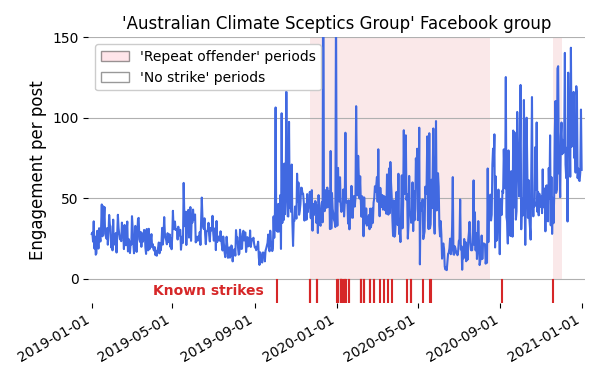
\includegraphics[width=\linewidth]{./../figure/repeat_example_timeseries.png}
\caption{Average engagement (the sum of comments, shares, likes, ...) per post for the `Australian Climate Sceptics Group' Facebook group for each day in 2019 and 2020. Each red line at the bottom represents the date of a known strike for this group, and the areas shaded in red represent the `repeat offender' periods as defined by the ‘two strikes in 90 days’ rule.}
\label{repeat_example_timeseries}
\end{figure}

To provide a general overview, we calculate the percentage change between the `repeat offender' and the `no strike' periods for each of the 256 Facebook accounts that have published at least one post during each period (see Figure \ref{repeat_vs_free_percentage_change}).\footnote{The percentage changes were calculated on the periods between January 1, 2019 and June 8, 2020. Because of the drop in engagement described further, the second semester of 2020 was excluded for its vastly diminished and not representative engagement level (see Figure \ref{repeat_average_timeseries}).}
The average percentage change is $7\%$, and the median $-6\%$. 
A Wilcoxon test shows that the values are not significantly different from zero (W = $16051$, p-value = $0.74$).

When we consider groups and pages separately, the percentage changes are different for the two. 
The median percentage change for Facebook groups is $-3\%$ (not significantly different from zero), while the median for Facebook pages is $-43\%$. 
A Wilcoxon test applied only to the Facebook pages' percentage changes, shows they are significantly different from zero (W = $21$, p-value = $0.0034$).

\begin{figure}[!h]
\centering
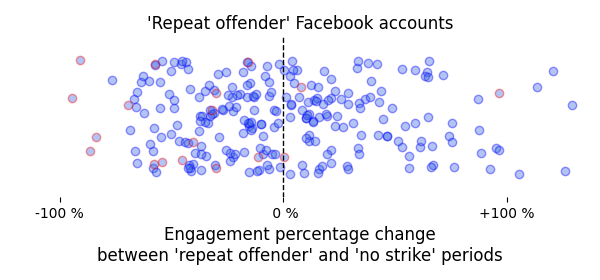
\includegraphics[width=\linewidth]{./../figure/repeat_vs_free_percentage_change.png}
\caption{Percentage changes between the average engagement per post during the `repeat offender' periods and the `no strike' periods. 
Each deep blue dot represents a Facebook group, and each light blue dot a Facebook page.
The bars show the medians for each set and their $90\%$ confidence intervals.
Confidence intervals are estimated using a bootstrap method.}
\label{repeat_vs_free_percentage_change}
\end{figure}

To see whether the strikes would otherwise influence the repeat offenders accounts' engagement over time, we analyzed the total amount of engagement received by all the posts published by each of the 307 repeat offenders accounts for each day of the 2019-2020 period (Figure \ref{repeat_average_timeseries}). 
This metric, representing the total engagement generated by these accounts on Facebook (top panel), can be decomposed as the number of posts published each day (middle panel) times the average number of engagement per post (bottom panel).

The total engagement per day is stable from January to September 2019, however we observe a rise from September 2019 to June 2020. 
This rise is explained by the increase in activity of the misinformation accounts (with a doubling of the number of posts per day) while the engagement per post remained rather constant.
Around June 9, 2020, the total engagement metrics have massively dropped.
This decrease is entirely explained by a corresponding drop in engagement per post (Figure \ref{repeat_average_timeseries}).

\begin{figure}[!h]
\centering
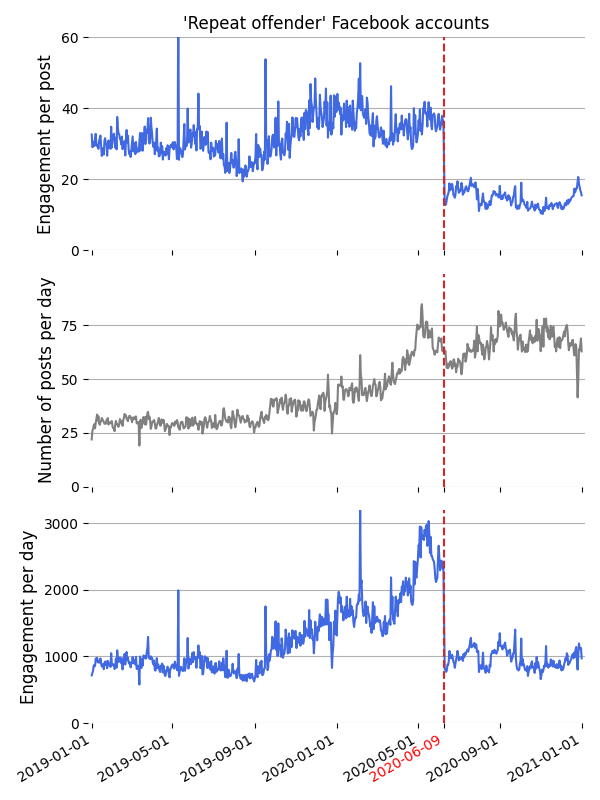
\includegraphics[width=\linewidth]{./../figure/repeat_average_timeseries.png}
\caption{
Metrics aggregated over the 307 Facebook accounts that repeatedly shared false news links. 
{\bf(Top panel)} Average engagement per day. 
{\bf(Middle panel)} Number of posts per day. 
{\bf(Bottom panel)} Average engagement per post. 
The dotted red line marks the date of June 9, 2020, when a sudden drop in engagement is observed.}
\label{repeat_average_timeseries}
\end{figure}

To further quantify this ‘June drop’, we calculated the percentage change in engagement for each account during a 30-day period before and after June 9, 2020 (Figure \ref{repeat_june_drop_percentage_change}). 
The average percentage change is $-21\%$, and the median $-43\%$. 
Most of the accounts (219 out of 289) experienced a decrease in engagement\footnote{A decrease in engagement on June 9, 2020 can be seen for the `Australian Climate Sceptics Group' in Figure \ref{repeat_example_timeseries} (the percentage change was $-60\%$ for this example).},
and a Wilcoxon test indicates that these percentage changes are significantly different from zero (W = $9012$, p-value = $4.6 \times 10^{-17}$).

It appears that the Facebook pages are not affected by this decrease, with a median percentage change of $-5\%$, while the groups have a median percentage change of $-45\%$. 
When tested separately, the Facebook pages' percentage changes are not significantly different from zero (W = $73$, p-value = $0.61$).

\begin{figure}[!h]
\centering
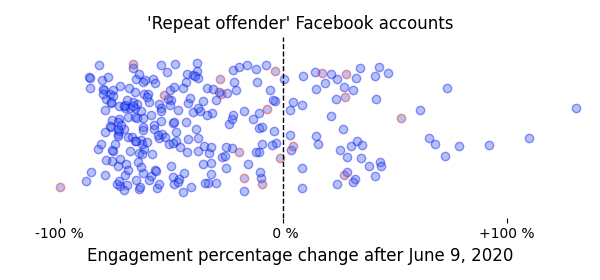
\includegraphics[width=\linewidth]{./../figure/repeat_june_drop_percentage_change.png}
\caption{Percentage changes in the average engagement per post during a 30-day period before and after June 9, 2020. 
Each deep blue dot represents a Facebook group, and each light blue dot a Facebook page.
The bars show the medians for each set and their $90\%$ confidence intervals.
}
\label{repeat_june_drop_percentage_change}
\end{figure}

To verify whether this drop was specific to this set of groups, we compared these dynamics to those of a control set of accounts consisting of Facebook pages and groups associated with established news outlets that did not publish misinformation.
No such drop in total or per post engagement metrics was observed around June 9, 2020.

We can only explain such a massive change by a modification in how Facebook’s algorithm promoted the content from these groups starting on June 9, 2020.
While we did observe a relationship between the strike dates and a decrease in engagement for `repeat offenders' pages, we observed no such link for `repeat offenders' groups.
Hence it seems that Facebook only took action against these groups via this one-shot measure in June.

One limitation of the results described in this section is that we obtained the links labelled as `False' from only one fact-checking organization (Science Feedback), while Facebook partners with over 60 fact-checking organizations\footnote{https://about.fb.com/news/2020/04/covid-19-misinfo-update/}.
The true `repeat offender' periods could thus be longer than the ones inferred, potentially changing the magnitude of the ‘reduce’ effect.

\section{Investigating the `reduce' policy on self-declared `repeat offenders'}

In the present section, we used a different methodology to collect accounts for which we are sure that they are under `repeat offender' status. 

\subsection{Methods}

We noticed that two popular pages (`Mark Levin' and `100 Percent FED Up') have publicly shared a message claiming to be placed under `repeat offender' status with a screenshot as a piece of evidence.
To gather a list of such self-declared repeat offenders, we searched on CrowdTangle for posts published since January 1, 2020 with the following keywords:
\begin{itemize}
\item `reduced distribution' AND (`restricted' OR `censored' OR `silenced')
\item `Your page has reduced distribution'
\end{itemize}
For this we used the `/posts/search' endpoint of the API on November 25, 2020. 

We manually opened the resulting posts, and kept the ones which met the following criteria (see Figure \ref{reduce_example} top panel for an example):
\begin{itemize}
\item The post should include a screenshot of the Facebook notification.
\item In the screenshot, the Facebook notification should say: `Your page has reduced distribution and other restrictions because of repeatedly sharing of false news.'
\item In the screenshot, the name of the page should be visible.
\end{itemize}

Doing so, we obtained a list of 94 pages. 
We found only Facebook pages in this case, and no groups. 
A search using the terms `Your group has reduced distribution' did not yield any result.

To verify whether Facebook applied any restriction to these pages, we collected all the posts that these 94 pages have published between January 1, 2019 and December 31, 2020 from the CrowdTangle API using the `/posts' endpoint. 
The collection was run on January 11, 2021.
We were only able to collect data from 83 of these pages, as 11 were deleted from the CrowdTangle database since our search in November 2020. 
This highlights an important issue when studying misinformation trends on Facebook: some data disappears as accounts are deleted or changed to ‘private’.

The date of the last notification was used as the inferred start date of reduced distribution, when it appeared in the screenshot. 
When it was not visible, we used the date of the post as the inferred start date of reduced distribution. 

\subsection{Results}

Figure \ref{reduce_example} shows a screenshot of the Facebook notification shared by the ‘I Love Carbon Dioxide’ page on April 28, 2020, and the average engagement per post of that page over the past two years. 
The engagement does not appear to be reduced after April 28, 2020. 
When we compare the engagement during a 30-day period before and after this date, the percentage change is $2\%$, indicating that the engagement is not affected by the `repeat offender' status.

\begin{figure}[!h]
\centering
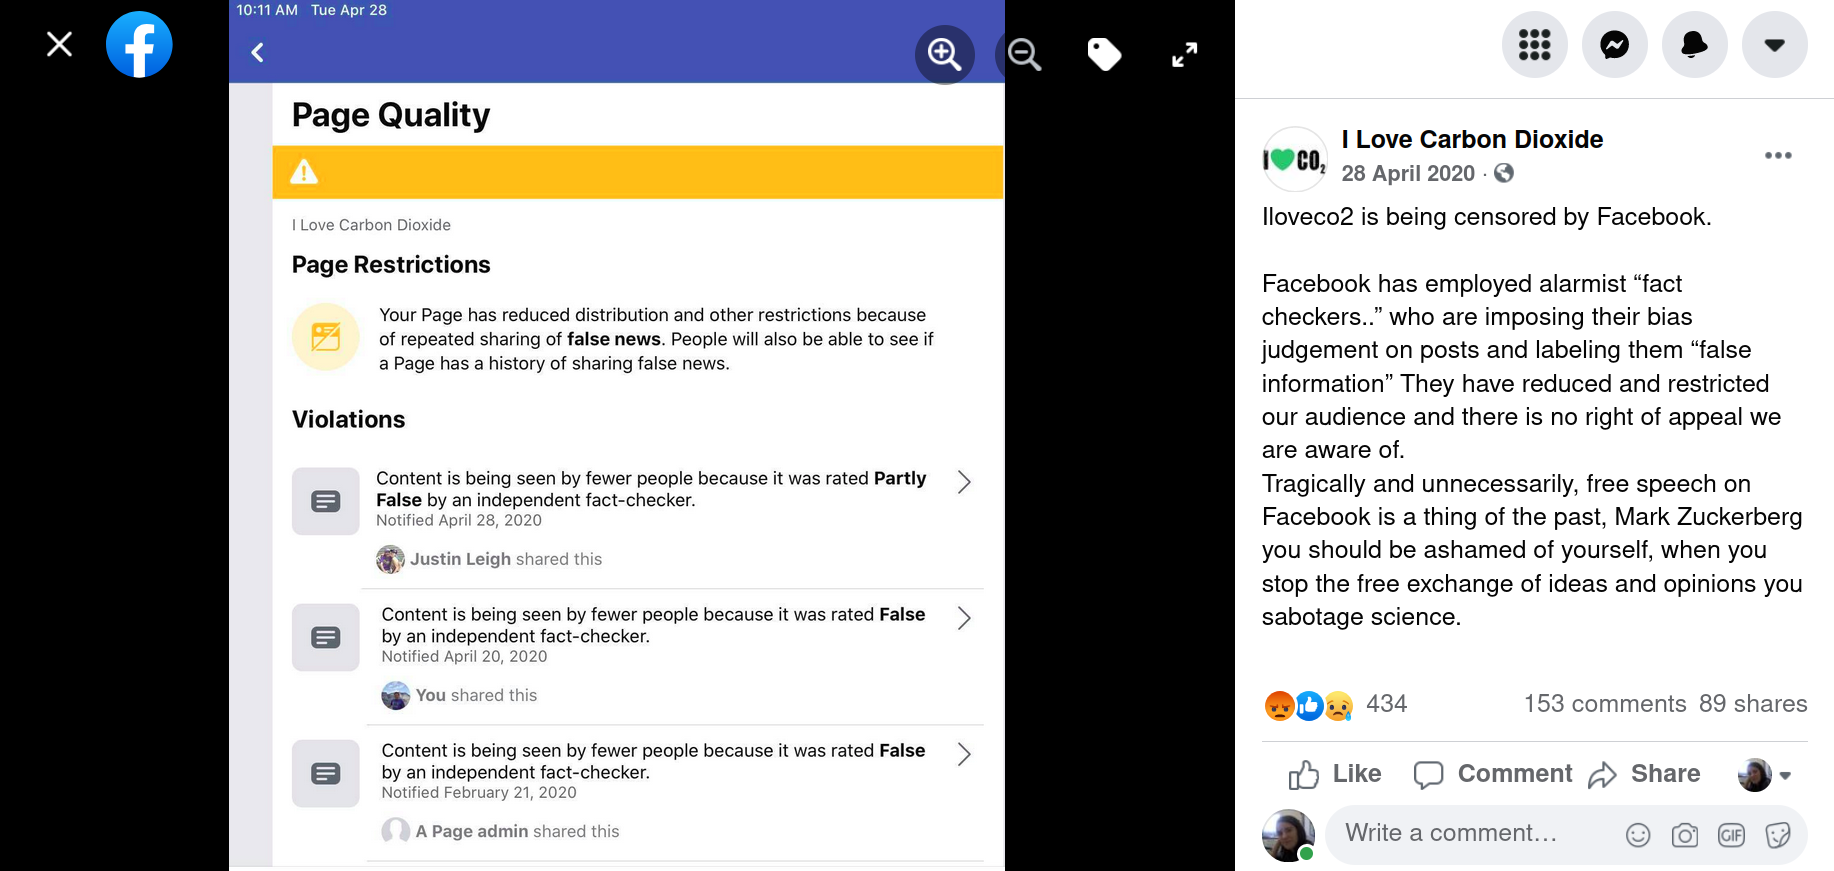
\includegraphics[width=\linewidth]{./../figure/reduce_example_screenshot.png}
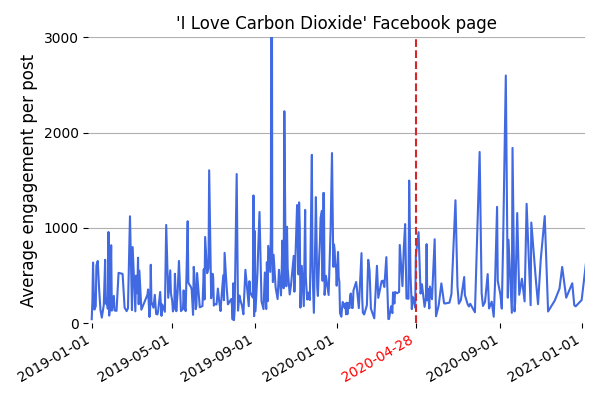
\includegraphics[width=\linewidth]{./../figure/reduce_example_timeseries.png}
\caption{
{\bf(Top panel)} Screenshot of a \href{https://archive.is/ie4dR}{post from the `I Love Carbon Dioxide' Facebook page} sharing a `reduced distribution' notification from Facebook. 
{\bf(Bottom panel)} Average engagement per post for the “I Love Carbon Dioxide” page for each day in 2019 and 2020.
The dotted red line represents the reduced distribution start date.}
\label{reduce_example}
\end{figure}

To provide a general overview, we calculate the percentage change in engagement during a 30-day period before and after the reduced distribution start date for each of the 82 Facebook pages that published at least one post during each period (see Figure \ref{reduce_percentage_change}).
The average percentage change is $-16\%$, the median is $-24\%$, and a Wilcoxon test reveals that the percentage changes are significantly different from zero (W = $911$, p-value = $0.00026$).
We can thus suggest that the `reduced distribution' status is associated with a modest decrease in engagement. 

However, there is a large heterogeneity across the different Facebook pages. The engagement of some popular pages have actually increased following the notification, such as the `Tucker Carlson Tonight' page with a $38\%$ increase (from 104k to 143k interactions per post).

\begin{figure}[!h]
\centering
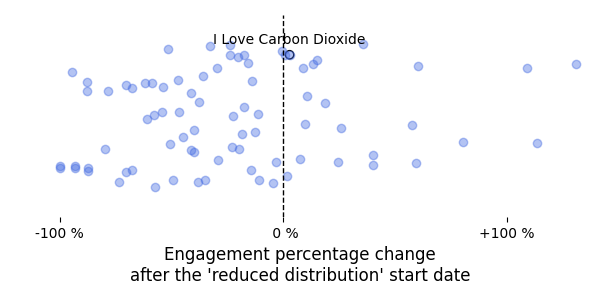
\includegraphics[width=\linewidth]{./../figure/reduce_percentage_change.png}
\caption{
Percentage changes in average engagement per post during a 30-day period before and after the reduced distribution start date. 
Each dot represents a Facebook page. 
The bars show the median and its $90\%$ confidence interval.
}
\label{reduce_percentage_change}
\end{figure}
 
Finally, we verify whether an important drop in engagement also occurred in June 2020 for this set of Facebook pages.
When we compare the engagement metrics before and after June 9, 2020, the percentage changes are not significantly different from zero (W = $1093$, p-value = $0.055$), and the median percentage change is $3\%$.
This confirms that Facebook pages have most likely not been affected by the {\it reduce} measure implemented on June 9, 2020 and evidenced in the previous section.

\section{Discussion}

Facebook, the most widely used social media platform in the world, has announced a series of measures to curb the spread of misinformation, notably by reducing the visibility of `repeat offenders', which are accounts that repeatedly share false information. 
However, the effects of the platforms' diverse policies to tackle misinformation remains understudied \citep{pasquetto2020tackling}. 
The present research article aims to contribute to filling this knowledge gap by verifying the application and measuring the consequences of Facebook's `reduce' policy on the targeted accounts' engagement metrics.

As a first step, we investigated the reach of 307 Facebook accounts (mainly groups) having repeatedly shared misinformation using a fact-checker's dataset. 
Sharing two false links over a three-month period is supposed to be penalized by a reduced visibility of the account's content. 
We did observe a significant decrease (median of $-43\%$) in the engagement per posts published by pages under a presumptive repeat offender status.
However, we find no evidence that this policy is leading to a significant decrease in engagement for Facebook groups.
 
As a second step, we identified 83 Facebook pages which have shared a Facebook notification, indicating that their account was under reduced distribution.
The pages' engagement metrics were significantly lower after the date of the notification (median of $-24\%$), suggesting that the `reduced distribution' measure was indeed applied to the pages.
We noted that no group was found when searching for accounts sharing a reduced distribution notification, which confirms that the `repeat offender' policy is applied only to Facebook pages, and not to groups.

By analyzing the time series of the repeat offenders’ engagement over the past two years, we also discovered a sudden drop affecting the groups around June 9, 2020.
For many groups, the decrease was quite drastic (up to $70\%$ - $80\%$), with a median drop in engagement of $45\%$.
The 18 Facebook pages from the first sample, as well as the 83 pages from the second sample, were not affected by this decrease.
This `June drop' does not correspond to any official communication by Facebook on that matter. 
It indicates that the company has very likely taken internal decisions that heavily impact the organic reach of repeat offenders' groups, in ways that differ from its stated policy against repeat offenders pages.
More transparency from Facebook would be needed to understand the nature and origin of this change. 
It would also bring clarity on how rules aimed at limiting the spread of misinformation are being enforced.

Facebook pages and groups have different purposes: pages are meant to be for official communication from the page administrators to a large audience, while groups are meant to foster interactions between users.\footnote{https://www.facebook.com/help/337881706729661/} 
Pages are thus always public, while groups can be public or private.
Pages' posts can also be monetized and promoted.
Despite these differences, both pages and groups are being used to spread false news. 
In the interest of curbing the spread of misinformation, applying its `repeat offender' policy to groups as well as to pages would help Facebook decrease the amount of misinformation in their users’ feeds. 
It is also not clear why only repeat offender Facebook groups, and not pages, saw their engagement reduced in June 2020.
Studies have highlighted that misinformation persists at high levels on Facebook and other platforms \citep{kornbluh2020new, resnick2018iffy}.
In the context of the COVID-19 pandemic, concerns rose about the amount of misinformation spreading on social media, including Facebook, and its potential harm to users \citep{johnson2020online}.
It is possible that such concerns have driven Facebook to apply a `quick fix' to decrease the engagement of posts shared in groups spreading misinformation and compensate for the absence of a repeat offender policy.
One should note that since the overall activity in these misinformation groups doubled between September 2019 and June 2020, the `June drop' has only succeeded in bringing the overall engagement level back to its early 2019 values (see Figure \ref{repeat_average_timeseries} top panel).

Online misinformation can be a threat to society, and the role that platforms can play via targeted interventions, has been the subject of intense debate over the past few years \citep{rogers2020deplatforming, de2020internet}. 
As a consequence, researchers \citep{mena2020cleaning, yaqub2020effects} and journalists\footnote{https://www.economist.com/graphic-detail/2020/09/10/facebook-offers-a-distorted-view-of-american-news, https://www.nytimes.com/2020/11/24/technology/facebook-election-misinformation.html} have begun to monitor the actions that platforms take to tackle misinformation and their efficacy.
Given the facts that 1) false news go viral much faster than fact-checks can get published, 2) accounts that have shared misinformation in the past tend to keep sharing misinformation and 3) a small number of accounts is responsible for a large proportion of the misinformation being shared (at least regarding COVID-19\footnote{https://www.counterhate.com/disinformationdozen}), acting against `repeat offenders' is likely to be one of the most effective interventions that platforms can make to protect their users against manipulation.

There is a critical need for further research to thoroughly verify and shed light on platforms' actions against misinformation. 
While our results provide information on the relative drop in engagement per post resulting from Facebook’s repeat offenders policy, more research is needed to quantify the impact of such policies on the overall prevalence of misinformation in users’ feeds.
 
\bibliography{biblio}
\bibliographystyle{acl_natbib}

\end{document}
